\documentclass[english, no-theorem-numbers]{short-notes}

\usepackage{math-alg,math-ag}

\addbibresource{math.bib}
%\bibliography{math.bib}

\title{new geometric techniques in number theory:\\spectral geometry of hecke algebras and traces}
\author{David Nadler\\Notes by Clemens Koppensteiner}
\date{Berkely, July 1--8, 2013}
\version{0}

\begin{document}

\newcommand\Sing{\operatorname{Sing}}
\newcommand\Loc{\operatorname{Loc}}
\newcommand\K{\sheaf K}%
\newcommand\ld[1]{\check{#1}}
\renewcommand\Gr{\operatorname{Gr}}
\newcommand\IC{\operatorname{IC}}
\newcommand\Bun{\operatorname{Bun}}

\maketitle

\tableofcontents
\bigskip\noindent
By geometry we mean that we work in the function field case, with a base field $k$ of characteristic $0$.

\section{derived algebraic geometry}

While algebraic geometers ostensibly study solutions to polynomial equations, it has been long known that it is important to keep track of the actual equations instead of merely their solutions.
Hence we can say that Algebraic Geometry is the study of \emph{systems} of polynomial equations.
An example of our slogan \enquote{equations over solutions} is the importance of nilpotents.

General references for this section are the works of Toën--Vezzosi and Lurie.

\subsection[Three examples of \enquote{derived equations}]{three examples of \enquote{derived equations}}

\subsubsection{Intersection multiplicities}

Consider $\as 4 = \Spec k[x,y,z,w]$ and the subvarieties $X₁ = \{x = y = 0\} \cup \{z=w=0\} = \{xz=xw=yz=yw\}$ and $X₂ = \{x = z,\, y = w\}$.
Obviously, $X₁ \cap X₂ = \{0\}$.
However, if we perturb $X₂$ by a little bit, we get two points.

If we impose all equations for $X₁\cap X₂$, then we get $x² = xy = xy = y²$.
Note that we get $xy$ in two different ways: from $xw = 0$, $y = w$ and from $yz = 0$, $x = z$.
Thus the dimension of $\O_{X₁ \cap X₂}$ is $3$ instead of the expected $2$ in the perturbed, \enquote{transversal} situation.
Serre's intersection multiplicity formula tells us that 
\[ 2 = 3 - 1, \]
where the $1$ is the dimension of a $\Tor$.

\subsubsection{Base change}

Consider a Cartesian diagram
\[
    \begin{tikzpicture}
        \matrix[commutative diagram] (m) {
            X₁ ×_Y X₂ & X₂ \\
            X₁ & Y \\
        };
        \path[commutative diagram arrows]
            (m-1-1) edge node[above] {$p₂$} (m-1-2)
                    edge node[left] {$p₁$} (m-2-1)
            (m-1-2) edge node[right] {$f₂$} (m-2-2)
            (m-2-1) edge node[below] {$f₂$} (m-2-2);
    \end{tikzpicture}
\]
Base change is the statement that ${p₂}_*p₁^* = f₂^*{f₁}_*$ as functors $\catCoh{X₁} → \catCoh{X₂}$.
Here and in the rest of the document all categories of modules and all functors between them are automatically derived, even when not explicitly mentioned in the notation.

Unfortunately, base change fails even in simple situations.
\begin{Ex}
    Consider the diagram 
    \[
        \begin{tikzpicture}
            \matrix[commutative diagram] (m) {
                \{0\} ×_{\as 1} \{0\} & \{0\} \\
                \{0\} & \as 1 \\
            };
            \path[commutative diagram arrows]
            (m-1-1) edge (m-1-2)
                    edge (m-2-1)
            (m-1-2) edge (m-2-2)
            (m-2-1) edge (m-2-2);
        \end{tikzpicture}
    \]
    Classically, the upper left corner is simply equal to $\{0\}$ again.
    The functor $\catModules{k} → \catModules{k}$ around the upper left part of the diagram is simply the identity, while the functor around the lower right is given by tensoring with the complex $k[1]\oplus k$.
    Derived algebraic geometry will change the upper functor ($\id$ in this case) by changing the fiber product.
\end{Ex}

\begin{Exercise}
    Let $Q^3 = \{A ∈ M₂ : \det A = 0\}$.
    This has two canonical resolutions $Q^3_+$ and $Q³_-$ given by adding a line in the kernel or cokernel of the matrix (they are a basic example of a \enquote{flop}).
    Find the correct (derived) fiber product $\tilde Q = Q³_+ ×_{Q³} Q³_-$, so that base change holds.
    (You will need material discussed later in this section to do the exercise.)
\end{Exercise}

\subsubsection{Moduli problems}

Classically there are strange ambiguities, in particular for deformations.

\begin{Ex}
    Let $\mathcal M_n$ be the moduli space of two commuting operators on $k^n$.
    We can write $\mathcal M_n$ as a fiber product
    \[
        \begin{tikzpicture}
            \matrix[commutative diagram] (m) {
                \mathcal M_n & M_n^2 \\
                \{0\} & M_n \\
            };
            \path[commutative diagram arrows]
            (m-1-1) edge (m-1-2)
                    edge (m-2-1)
            (m-1-2) edge node[right] {$[\,{,}\,]$} (m-2-2)
            (m-2-1) edge (m-2-2);
        \end{tikzpicture}
    \]
    For $n = 1$ we obtain
    \[
        \begin{tikzpicture}
            \matrix[commutative diagram] (m) {
                \mathcal M₁ & \as 1 × \as 1 \\
                \{0\} & M₁ \\
            };
            \path[commutative diagram arrows]
            (m-1-1) edge (m-1-2)
                    edge (m-2-1)
            (m-1-2) edge node[right] {$[\,{,}\,]$} (m-2-2)
            (m-2-1) edge (m-2-2);
        \end{tikzpicture}
    \]
    and, since any two matrices in $M₁$ commute, that $\mathcal M₁ = \as 1 × \as 1$.
    But if we deform slightly and require that $[\,{,}\,] = λ \ne 0$, then the moduli space suddenly becomes empty!
\end{Ex}

\subsection[Local (affine) \textsc{dag}]{local (affine) dag}

Imposing equations translates to tensor products and in a derived setting this means that we have to keep track of $\Tor$s.

\begin{Def}
    A \emph{commutative differential-graded algebra} (\emph{cdga}) $A^\cx$ over $tk$ is a commutative, associative algebra in $k$-chain complexes.
\end{Def}

\begin{Rem}
    We consider cdgas only up to quasi-isomorphism, but be aware that $A^\cx$ knows more that $H^\cx(A^\cx)$.
\end{Rem}

\begin{Exercise}
    Give an example of two cdgas with the same cohomology algebra (hint: Massey products).
\end{Exercise}

\begin{Def}
    A \emph{derived ring} $A^\cx$ is a cdga which is connective, i.e.~$H^iA^\cx = 0$ for $i > 0$.
    The opposite category to derived rings is called the category of \emph{affine derived schemes}.
\end{Def}

\begin{Notation}
    We often write $π_i = H^{-i}$.
\end{Notation}

\begin{Rem}
    We have a canonical map $A^\cx → π₀A^\cx$.
    Hence we can view $A^\cx$ as a \enquote{derived thickening} of $π₀A^\cx$.
    On schemes, we see this as an embedding $\Spec π₀A^\cx \hookrightarrow \Spec A^\cx$.
\end{Rem}

The source of all examples for derived rings are iterated fiber products where we keep track of $\Tor$ complexes.

\subsubsection{Structure of cdgas}

The category of cdgas should be properly viewed as an $∞$-category and is a simplicial localization of a model category.
The main structure are simplicial sets of $\Hom$:
\[
    \Hom^n(A,B) = \Hom^0(A, B \otimes Ω^\cx(Δ^n)).
\]
Practically, to calculate derived operations we only need to know the following:
\begin{enumerate}
    \item All objects are fibrant.
    \item Cell cdgas are cofibrant.
\end{enumerate}

\begin{Def}
    A cdga $A$ is a \emph{cell cdga} if it has a filtration
    \[
        k = A_0 \hookrightarrow A₁ \hookrightarrow A₂ \hookrightarrow \dotsb \hookrightarrow A_n = A,
    \]
    such that $A_{i+1} = A_i[x_i]$ with $\deg x_i ∈ ℤ$ and $dx_i ∈ A_i$.
    \todo{Is this the same as semifree algebras?}%
    \todo{Rather than $k$ should we start with the algebra over which we are taking the tensor product?}%
\end{Def}

\begin{Ex}
    Consider a hypersurface $X = \{f = 0\}$ in $\as n$.
    Traditionally we have $\O(X) = \rquot{k[x₁,\dotsc,x_n]}{(f)}$.
    The cofibrant replacement of this is $k[x₁,\dotsc,x_n][ε]$ with $\deg ε = -1$ (and hence $ε²=0$) and $dε = f$.
\end{Ex}

\subsubsection{Linearization}

Let $A$ be a derived ring.

\paragraph{modules}
Attached to $A$ are various categories of modules, which are summarized in Figure~\ref{fig:modules}.
\begin{figure}[htb]
    \centering
    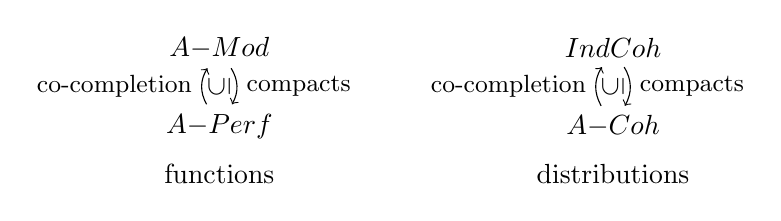
\begin{tikzpicture}
        \node (QCoh) at (0,0) {$A\text{-}\cat{Mod}$};
        \node at (0,-0.5) [rotate=90] {$\subseteq$};
        \node (Perf) at (0,-1) {$A\text{-}\cat{Perf}$};
        \draw[->] (Perf) to[bend left=30] node[left] {\small co-completion} (QCoh);
        \draw[->] (QCoh) to[bend left=30] node[right] {\small compacts} (Perf);
        \node at (0,-1.6) {\enquote{functions}};
        \begin{scope}[xshift={5cm}]
            \node (IndCoh) at (0,0) {$\cat{IndCoh}$};
            \node at (0,-0.5) [rotate=90] {$\subseteq$};
            \node (Coh) at (0,-1) {$A\text{-}\cat{Coh}$};
            \draw[->] (Coh) to[bend left=30] node[left] {\small co-completion} (IndCoh);
            \draw[->] (IndCoh) to[bend left=30] node[right] {\small compacts} (Coh);
            \node at (0,-1.6) {\enquote{distributions}};
        \end{scope}
    \end{tikzpicture}
    \caption{Categories of modules attached to a derived ring.}
    \label{fig:modules}
\end{figure}
\begin{itemize}
    \item $A\text{-}\cat{Mod}$ is the category of derived dg modules.
    \item $A\text{-}\cat{Perf}$ the subcategory consisting of summands of finite complexes of shifts of $A$.
    \item $\cat{IndCoh}$ is the category of ind-coherent modules.
    \item $A\text{-}\cat{Coh}$ is the subcategory of $A\text{-}\cat{Mod}$ consisting of complexes with bounded coherent cohomology.
\end{itemize}

\paragraph{cotangent complex}
To $A$ we attach its \emph{cotangent complex} $\mathbb L_A ∈ A\text{-}\cat{Mod}$, which is a connective module such that $π₀\mathbb L_A$ coincides with the cotangent bundle $Ω_{π₀A}$.
The universal characterization of the cotangent complex is 
\[
    \operatorname{Der}(A,M) = \Hom(\mathbb L_A, M).    
\]
In particular we have a \enquote{Kähler differential} $d\colon A → \mathbb L_A$.

To calculate we only need to know that $\mathbb L_A$ coincides with the cotangent bundle on smooth classical affine schemes and if $D = A \otimes_C^{\mathbb L} B$, then
\[
    \mathbb L_D = \operatorname{Cone}\left( \mathbb L_A \otimes_A D → (\mathbb L_B \otimes_B D) \oplus (\mathbb L_C \otimes_C D) \right),
\]
where the map is given by pullback.

\subsection[Global \textsc{dag}]{global dag}

We take the functor of points viewpoint:
\[
    \begin{tikzpicture}
        \matrix[commutative diagram] (m) {
            \cat{Aff}^{\mathrm{op}} & \cat{Sets} \\
            \cat{DAff}^{\mathrm{op}} & \cat{Spaces} = \cat{SSet} \\
        };

        \path[->] 
            (m-1-1) edge node[above] {Sch} (m-1-2)
                    edge node[auto,sloped,anchor={south}] {Stacks} (m-2-2)
            (m-2-1) edge node[below] {DStacks} (m-2-2);
        \path[right hook->]
            (m-1-1) edge (m-2-1)
            (m-1-2) edge (m-2-2);
    \end{tikzpicture}
\]
In particular, Artin derived stack are given by a diagram of the form
\[
    X \leftarrow \left(X₀ \leftleftarrows X₁\right),
\]
where $X₀$ and $X₁$ are derived schemes and the two arrows $\leftleftarrows$ are smooth maps.

\begin{Ex}\leavevmode
    \begin{enumerate}
        \item $BG \leftarrow (\mathrm{pt} \leftleftarrows G$), for $G$ a group.
        \item $M_{1,1} \leftarrow (? \leftleftarrows ?)$.
        \item $S¹ \leftarrow (\mathrm{pt} \leftleftarrows ℤ)$.
            \qedhere
    \end{enumerate}
\end{Ex}

\section{microlocal algebraic geometry}

The goal of this section is to introduce geometric Arthur parameters. 
There is work by many people on the ideas we will introduce, but the \enquote{state of the art} is \cite{ArinkinGaitsgory:arXiv:SingularSupport}.

We will work locally and set $X = \{F = 0\}$, where $F\colon \as n → \as k$.
We want to understand the (derived) category $\catCoh X$.

\subsection[Philosophy: two themes]{philosophy: two themes}

The ideas we will introduced a based on two major themes in mathematics. 
The first of these is illustrated by the following example.

\begin{Ex}
    Let $A$ be an algebra and consider the category $\catModules A$ of $A$-modules.
    Let $Z(A)$ be the center of $A$.
    Then $\Spec Z(A)$ is a scheme, and we can localize $A$ as a sheaf of algebras on $\Spec Z(A)$.
    Therefore we can localize the category $\catModules A$ on $\Spec Z(A)$.
\end{Ex}

More generally, if $\cat C$ is a category, we can sheafify $\cat C$ over $Z(\cat C) = \End(\id[\cat{C}])$.

The second theme is that there are two types of \enquote{geometric measurements}: 
\begin{itemize}
    \item static measurements corresponding to points of $X$, e.g.~talking stalks;
    \item dynamic measurements corresponding to $T^*X$, e.g.~taking vanishing cycles.
\end{itemize}

A classical example is Fourier transform $L²(S¹) \isoto L²(ℤ)$.

\subsection[Koszul duality]{koszul duality}

Let $V = \Spec k[x₁,\dotsc,x_n]$ with $\deg x_i = -1$ be a \enquote{vector space in degree $-1$.}
We want to analyze $\catCoh V$.

Note that $V_{\mathrm{cl}} = \Spec π₀V$ is just a point, so that this doesn't give us any way to localize.
Thus we introduce \emph{codirections} $V^*[1] = \Spec k[ξ₁,\dotsc,ξ_n]$ with $\deg ξ_i = 2$.

\begin{Thm}[Koszul Duality]
    There is an equivalence of categories
    \[
        \catCoh V \cong \catCoh{V^*[1]},
    \]
    sending the structure sheaf $\O_V$ to the skyscraper $k$ on $V^*[1]$ and the skyscraper $k$ on $V$ to $\O_{V^*[1]}$.
\end{Thm}

Thus we can localize coherent sheaves on $V$ on $V^*[1]$ (which is given by a \enquote{usual} polynomial ring).
Supports will be closed conic subvarieties.

\begin{Exercise}
    Under Koszul Duality, $\sheaf F ∈ \catCoh V$ is perfect if and only if $\supp F \subseteq \{0\} \subseteq V^*[1]$.
\end{Exercise}

\begin{Rem}
    We think of $\catCoh V$ as \enquote{distributions} and $\catPerf V \subseteq \catCoh V$ as \enquote{functions}.
    Koszul Duality measures the codirections on which \enquote{smoothness} fails.
\end{Rem}

\begin{Exercise}
    Show that $V = \{0\} ×_{\as n} \{0\}$ as derived schemes.
    Thus $V$ is an Abelian groupoid via \enquote{concatenation of paths}.
    This turns $\catCoh V$ into a tensor category with tensor product $*$ given by convolution.
    Show that Koszul Duality is an equivalence of tensor categories exchanging $*$ with the usual tensor product $\otimes$ in $\catCoh{V^*[1]}$.
\end{Exercise}

\subsection[The scheme of singularities]{the scheme of singularities}

Let us return to the situation of $X = \{F = 0\} \subseteq \as n$.
The cotangent complex of $X$ is given by
\[
    \mathbb L_X = \left( Ω_{\as k} \xrightarrow{dF^*} Ω_{\as n} \right)
\]
in degrees $-1$ and $0$.

\begin{Def}
    The (classical) scheme $\Sing(X) → X$ is the scheme with fiber at $x ∈ X$ given by $H^{-1}\mathbb L_X$.
\end{Def}

\begin{Ex}
    Consider $X = \{x³ = y²\}$.
    Then $\Sing(X)$ is the whole picture given in Figure~\ref{fig:SingEx}.
    \begin{figure}[htb]
        \centering
        \begin{tikzpicture}
            \draw plot[smooth] file {cusp.table};
            \draw[y=-1cm] plot[smooth] file {cusp.table};
            \draw (-1,0) -- (1.5,0);
        \end{tikzpicture}
        \caption{Scheme of singularities of $x³ = y²$}
        \label{fig:SingEx}
    \end{figure}
\end{Ex}

\begin{Rem}
    We always have $\Sing X \subseteq X × \as k$.
\end{Rem}

We can then localize $\catCoh X$ over $\Sing(X)$.

\begin{Rem}
    This will be the ultimate localization.
\end{Rem}

To do so, we need do find the action of $\O(\as k) = k[ξ₁,\dotsc,ξ_k]$.
Consider the Cartesian diagrams (in derived schemes)
\[
    \begin{tikzpicture}
        \matrix[commutative diagram] (m) {
            X & \as n \\
            \{0\} & \as k \\
        };
        \path[commutative diagram arrows]
            (m-1-1) edge (m-1-2) edge (m-2-1)
            (m-1-2) edge node[right] {$F$} (m-2-2)
            (m-2-1) edge (m-2-2);

        \begin{scope}[xshift={4cm}]
            \matrix[commutative diagram] (m) {
                V & \{0\} \\
                \{0\} & \as k \\
            };
            \path[commutative diagram arrows]
                (m-1-1) edge (m-1-2) edge (m-2-1)
                (m-1-2) edge (m-2-2)
                (m-2-1) edge (m-2-2);
        \end{scope}
    \end{tikzpicture}
\]
We should think of points of $X$ as paths from $F$ to $\{0\}$ and points in $V$ as loops based at $\{0\}$.
Thus we can concatenate such a path with a loop and get another path.

The upshot of this is that we have an action of $\catCoh V$ on $\catCoh X$.
The unit of the convolution product $*$ of $\catCoh V$ is $k$.
Hence we obtain a map
\[
    k[ξ₁,\dotsc,ξ_k] = \End(k) → \End(\id[\catCoh X]).
\]
In other words, $k[ξ₁,\dotsc,ξ_k]$ acts universally on every object of $\catCoh X$.
Hence $\catCoh X$ can be localized on $X × \as n$.

\begin{Exercise}
    The support of any element of $\catCoh X$ will always be contained in $\Sing(X)$.
\end{Exercise}

\begin{Ex}
    Let $Q³ = \{A ∈ M₂ : \det A = 0\}$.
    This can be presented as
    \[
    \begin{tikzpicture}
        \matrix[commutative diagram] (m) {
            Q³ & \as 4 \\
            \{0\} & \as 1 \\
        };
        \path[commutative diagram arrows]
            (m-1-1) edge (m-1-2) edge (m-2-1)
            (m-1-2) edge node[right] {$\det$} (m-2-2)
            (m-2-1) edge (m-2-2);
    \end{tikzpicture}
    \]
    and $\Sing(X) \subseteq X × \as 1$ is $X$ together with a one-dimensional \enquote{spoke} at the origin.
\end{Ex}

\begin{Exercise}
    Let $\sheaf F ∈ \catCoh X$.
    Show that $\supp \sheaf F \subseteq \{0\} \subseteq \Sing(X)$ if and only if $\sheaf F ∈ \catPerf X$.
\end{Exercise}

\subsection[Geometric Arthur parameters]{geometric arthur parameters}

In the function field setup, the analogue of the number field in the Langlands program is a smooth projective curve $C$ over the ground field $k$.
The analogue of a Galois representation is then a local system for $G$ (or rather $\ld G$, but we will only talk about one side of the correspondence for now, so we omit the dual for simplicity).
We write $\Loc_G(C)$ for the moduli of local $G$-systems on $C$.

A common source of confusion here is that there are two notions of local systems in the geometric context:
\begin{itemize}
    \item The \enquote{Betti version}: A local system is a representation of the fundamental group of $C$, i.e. a map $π₁(C) → G$.
        This looks most immediately like a Galois representation: the fundamental group is the geometric analogue of the Galois group in the number field setting.
    \item The \enquote{de Rham version}: A local system is a $G$-bundle with a flat connection.
\end{itemize}
These two notions are analytically equivalent, but not algebraically equivalent.
So their local geometry is the same, but there are global aspects where they differ.

For simplicity, we will only consider the Betti version in this lecture.
Thus we set
\[
    \Loc_G(C) = \rquot{\left\{ π₁C → G  \right\}}{G}.
\]
This is a nice Artin stack.
Let us describe it in more detail.
First, if we pick a point in $C$ and trivialize a $G$-bundle we get rid of the symmetries.
Hence we get a presentation of $\Loc_G(C)$ as the groupoid\todo{So $\Loc_G(C)'$ is the moduli of local systems trivialized at a point of $C$?}
\[
    \Loc_G(C) \leftarrow \left( \Loc_G(C)' \leftleftarrows G \right).
\]
Let $g$ be the genus of $C$ (so $2g$ is the number of generators of $π₁(C)$).
We can further write $\Loc_G(C)'$ as the fiber product
\[
    \begin{tikzpicture}
        \matrix[commutative diagram] (m) {
            \Loc_G(C)' & G^{2g} \\
            \{1\} & G \\
        };
        \path[commutative diagram arrows]
            (m-1-1) edge (m-1-2) edge (m-2-1)
            (m-1-2) edge node[right] {$[\,{,}\,]$} (m-2-2)
            (m-2-1) edge (m-2-2);
    \end{tikzpicture}
\]
where $[\,{,}\,]$ is the commutator map\todo{How to define the commutator map $G^{2g} → G$?}. 
In other words, we take the curve, puncture it, take a local system on the punctured curve which will have $2g$ monodromies and ask that it extends over the puncture, i.e. the commutator is $1$.

Now we have a diagram as before (with $F = [\,{,}\,]$).
The spaces $G$ and $G^{2g}$ are not affine, but they are still nice smooth varieties.
Hence, if we ignore the $G$-symmetries, $\Loc_G(C)$ looks like the kind of complete intersections we studied in the first part of this section.

We can now define the geometric analogue of Arthur's parameters: they are $\Sing(X)$ for this stack, i.e. we call
\[
    \Sing(\Loc_G(C)) \subseteq \rquot{(\Loc_G(C)' × \liealg g^*)}{G}
\]
the \emph{moduli of geometric Arthur's parameters}.
Note that $\liealg g^*$ appears for the cotangent space (as $G$ is not affine).
One expects that automorphic objects lead to coherent sheaves with nilpotent Arthur's parameters.
\todo{Interpretation}

\section{geometry of hecke categories -- satake correspondence}

The goal of this section is discuss a geometric verison of the Satake correspondence.
A lot of the material we will talk about has been very well understood for the last two decades, but by the end we will talk about something new that will tie in with the last two sections.
The goal is to give an introduction to geometric techniques for understanding Hecke categories -- specifically spherical Hecke categories.

\subsection[Reminder on the Satake correspondence]{reminder on the satake correspondence}

Let $G$ be a reductive group.
As we will soon move to characteristic $0$, so for simplicity we assume that $G$ is defined over $ℤ$.
Attached to $G$ is its root datum
\[
    \left( Λ_G,\, \ld{Λ}_G,\, R_G, \ld R_G \right),
\]
consisting of the coweight lattice (homomorphisms from $\mathbb G_m$ into a maximal torus of $G$), the weight lattice (the dual), the coroots and the roots of $G$.
Switching weights and coweights and roots and coroots, we obtain the \emph{Langlands dual group} $\ld G$ of $G$.
\begin{Ex}
    The Langlands dual of $\GL n$ is again $\GL n$.
    The Langlands dual of $\SL n$ is $\PGL n$.
\end{Ex}

Recall that the \emph{spherical Hecke algebra} of $G$ consists of the compactly supported functions on $G(ℚ_p)$ which are $G(ℤ_p)$-biinvariant, i.e.
\[
    H_{\mathrm{sph}} = ℂ_c\biggl[ \dquot{G(ℤ_p)}{G(ℚ_p)}{G(ℤ_p)} \biggr].
\]
The \emph{Satake correspondence} identifies this with functions on the Langlands dual group.
More concretely it is an isomorphism 
\begin{equation}
    \label{eq:Hecke:Satake}%
    H_{\mathrm{sph}} \cong \O(\ld G)^{\ld G}
\end{equation}
of commutative algebras between the spherical Hecke algebra of $G$ (with convolution $*$; we won't discuss the definition here, but see the geometric version below) and the representation ring of $\ld G$ (with multiplication $\cdot$).
One can think of this as a kind of Fourier transform: it identifies something that is not evidently commutative with functions on something.

The goal of this section is to discuss a geometric version of the Satake isomorphism: 
We are going replace the algebras be symmetric monoidal categories of sheaves.
Thus we get a statement with a lot more structure, that allows one to use the tools from algebraic geometry (e.g.~Hodge theory).
So on the one hand the geometric version will be a more complicated statement than \eqref{eq:Hecke:Satake}, but on the other hand its additional structure gives a richer, more powerful statement.
In particular, \eqref{eq:Hecke:Satake} can then be deduced from the categorical version.

\subsection[The affine Grassmannian]{the affine grassmannian}

Note that in the definition of the spherical Hecke algebra we could have used any local with finite residue field instead of $ℚ_p$.
For example, we could have defined it over $\mathbb F_p\lParen t \rParen$, already putting us into the function field case in the Satake correspondence.
In the geometric case, we replace $\mathbb F_p$ by an algebraically closed field.
Specifically we will use the complex numbers and from now on let $k = ℂ$ (although one could also take $k = \overline{\mathbb F_p}$ and reproduce everything that follows).

To simplify notation, we let $\K = k\lParen t \rParen$ be the ring of Laurent series over $k$ and $\O = k\lBrack t \rBrack$ its subring of power series.
As replacement of $G(ℚ_p)$ in the $p$-adic case we take the \emph{loop group} $LG = G(\K)$
This will have a structure of a $k$-variety, but for the moment we just think of $LG$ as a set.
For example, if $G = \GL n$, then $G(\K)$ consists of invertible matrices with coefficients in $\K$.
Further we define the \emph{arc group} $L_+G = G(\O)$.

The names of these objects come from the following interpretation.
On can think of $ℚ_p$ as a little punctured disc around $p$ in $\Spec ℤ$ and the same is true for Laurent series: you get them when you look at a little punctured disc around a point on a curve.
So we think of $\Spec \O$ as a formal disc and $\Spec \K$ as a punctured formal disc.
Thus elements of $LG$ are maps from a punctured disc into $G$, i.e. \enquote{loops}.

\begin{Def}
    The \emph{affine Grassmannian} (or \emph{loop Grassmannian}) is
    \[
        \Gr = \Gr_G = \rquot{LG}{L_+G}.
    \]
    as a set.
\end{Def}
The name comes from the fact that $LG$ is an affine Kac-Moody group with maximal parabolic $L_+G$ and hence one can think of $\rquot{LG}{L_+G}$ as a kind of flag variety.

The key structure that the affine Grassmannian has -- that one doesn't have for $\rquot{G(ℚ_p)}{G(ℤ_p)}$ -- is that it is naturally an increasing union of projective varieties.

\begin{Ex}
    Let $G = \GL n$.
    Then we have an action of $L\GL n$ on $\K^n$.
    The basic lattice $\O^n \subseteq \K^n$ (see Figure~\ref{fig:GLnlattice}) is preserved by $L_+\GL n$.
    \begin{figure}[htb]
        \centering
        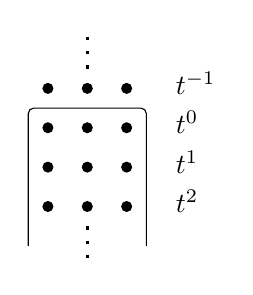
\begin{tikzpicture}[y={-0.5cm}, x={0.5cm}]
            \foreach \i in {-1,0,1,2} {
                \foreach \j in {-1,0,1} {
                    \fill ({\j},{\i}) circle[radius=2pt];
                }
                \node[anchor=mid west] at (2,\i) {$t^{\i}$};
            }
            \draw[rounded corners=2pt] (-1.5,3) -- (-1.5,-0.5) -- (1.5,-0.5) -- (1.5,3);
            \draw[loosely dotted, very thick] (0,-1.5) -- (0,-2.5);
            \draw[loosely dotted, very thick] (0,2.5) -- (0,3.5);
        \end{tikzpicture}
        \caption{The lattice of basis vectors of $\K^3$ after fixing a basis for $ℂ³$ with the basic lattice $\O^3$ marked.}
        \label{fig:GLnlattice}
    \end{figure}
    \begin{Exercise}
        Show that 
        \[
            \Gr_{\GL n} = 
            \left\{ 
                \text{$k$-subspaces $W \subseteq \K^n$ such that $tW \subseteq W$ and $t^N\O^n \subseteq W \subseteq t^{-N}\O^n$ for $N \gg 0$}
            \right\}.
        \]
        (Hint: check that the loop group acts transitively on the lattices and the arc group preserves the basic lattice.)
    \end{Exercise}
    As a consequence of the exercise, we can write 
    \[
        \Gr_{\GL n} = \smash{\bigcup\limits_{\mathclap{N = 0}}^∞ \Gr_N},
    \] 
    with
    \[
        \Gr_N = 
        \left\{ 
            \text{$k$-subspaces $W \subseteq \K^n$ such that $tW \subseteq W$ and $t^N\O^n \subseteq W \subseteq t^{-N}\O^n$}
        \right\}.
    \]
    See Figure~\ref{fig:GLnlatticeN} for an illustration of $\Gr_2$.
    
    \begin{Exercise}
        Check that each $\Gr_N$ is a projective variety.
    \end{Exercise}
    
    \begin{figure}[htb]
        \centering
        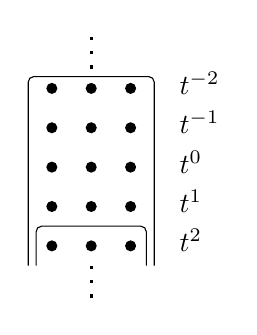
\begin{tikzpicture}[y={-0.5cm}, x={0.5cm}]
            \foreach \i in {-2,-1,0,1,2} {
                \foreach \j in {-1,0,1} {
                    \fill ({\j},{\i}) circle[radius=2pt];
                }
                \node[anchor=mid west] at (2,\i) {$t^{\i}$};
            }
            \draw[rounded corners=2pt] (-1.6,2.5) -- (-1.6,-2.3) -- (1.6,-2.3) -- (1.6,2.5);
            \draw[rounded corners=2pt] (-1.4,2.5) -- (-1.4,1.5) -- (1.4,1.5) -- (1.4,2.5);
            \draw[loosely dotted, very thick] (0,-2.5) -- (0,-3.5);
            \draw[loosely dotted, very thick] (0,2.5) -- (0,3.5);
        \end{tikzpicture}
        \caption{The bounds for $W$ in $\Gr_2$.}
        \label{fig:GLnlatticeN}
    \end{figure}
\end{Ex}

We are going to study the topology of this increasing union of finite dimensional projective varieties.

\subsection[Alternative descriptions]{alternative descriptions}

There are a couple of other useful ways to think about the affine Grassmannian.

\subsubsection{Bundles}

Let $D = \Spec \O$ and $D^× = \Spec \K$.

\begin{Exercise}
    Show that the Grassmannian $\Gr_G$ is the set of $G$-bundles on $D$, trivialized on $D^×$.
\end{Exercise}

Let $\mathbb D = D \amalg_{D^×} D$ is the disc with two zeros.
\begin{Exercise}
    Show that
    \[
        \lquot{L_+G}{\Gr} =
        \dquot{L_+G}{LG}{L_+G} = 
        \{ \text{$G$-bundles on $\mathbb D$}\}.
    \]
\end{Exercise}

The reason that this description is useful is that in Geometric Langlands the automorphic moduli space is a space of bundles.

\subsubsection{Topological}

Let $K \subseteq G$ be a maximal compact and let $ΩK$ be the based polynomial\footnote{I.e., as maps $S¹ → K$ the loops have finite Fourier expansion} loop group on $K$.

\begin{Exercise}
    Show that
    \[ \Gr \cong ΩK\]
    as topological spaces.
    (Hint: Show that $LG \cong ΩK × L_+G$.)
\end{Exercise}

Note that this gives $\Gr$ the structure of a group (though not of an \emph{algebraic} group).

\begin{Exercise}
    Show that for $G = \PGL 2$ one has
    \[
        \Gr_{\PGL 2} = \rquot{\operatorname{Free}(S²)}{xa(x) = 1},
    \]
    where $\operatorname{Free}(X)$ denotes the free topological group on $X$ and $a\colon S² → S²$ is the antipodal map.
\end{Exercise}

\subsection[A little structure theory]{a little structure theory}

We have the following analogues of $p$-adic structure theory.

\subsubsection{Cartan decomposition}

There is an isomorphism of sets
\[
    \lquot{L_+G}{\Gr} =
    \dquot{L_+G}{LG}{L_+G} \cong
    \rquot{Λ_G}{W} \cong
    Λ_G^+,
\]
where $W$ is the Weyl group and $Λ^+_G$ the dominant coweights.
Note that $Λ^+_G$ is also the dominant weights of the Langlands dual group.
So this is a first hint that the geometry of this space will have something to do with the dual group, i.e.~we can interpret this as a first hint of Langlands duality.


\subsubsection{Iwasawa decompostition}

There is an isomorphism of sets
\[
    \lquot{N(\K)}{\Gr} = \dquot{N(\K)}{LG}{L_+G} \cong Λ_G,
\]
where $N$ is the unipotent radical of a Borel of $G$.

\todo{34:00--41:00 (Example of $\PGL 2$).}

\subsection[Geometric Satake]{geometric satake}

\subsubsection{Geometric \texorpdfstring{$L_+G$}{L+G}-invariant \enquote{distributions} on \texorpdfstring{$\Gr$}{Gr}}


We want to consider $L_+G$-equivariant \enquote{geometric distributions} on $\Gr$.
The function--sheaf correspondence tells us that a good way to obtain constructible functions on a variety is to look at sheaves and take traces of Frobenius. 
This hints that to get a more structured version of \enquote{functions}, one should pass to constructible sheaves.
This is exactly what we are going to do now without further justification.

So we are going to pass to the category $\cat P_{L_+G}(\Gr)$ of $L_+G$-equivariant perverse sheaves on $\Gr$\todo{Intro to perverse sheaves.}.
This category is Abelian (always) and semisimple (in this situation!).
The simple objects are given by the intersection complexes $\IC^λ = \IC(\Gr^λ)$, where $\Gr^λ \subseteq \Gr$ is the closure of the $L_+G$-orbit indexed by $λ ∈ \rquot{Λ_G}W$.
This is the \enquote{best basis of the Hecke algebra.}

The first hint of Satake are the following equations due to Lustzig.
Let $V^λ$ be the irreducible representation of $\ld G$ of highest weight $λ ∈ \rquot{\ld Λ_{\ld G}}W = \rquot{Λ_G}W$.
Then,
\[ 
    \dim \mathrm RΓ(\Gr,\, \IC^λ) = \dim V^λ
\]
and
\[
    \dim \res{\IC^λ}μ = \dim \operatorname{wt}_μ(V^λ)
\]
for any point $μ$ in $\Gr^λ$.

\begin{Thm}[Geometric Satake \cite{MirkovicVilonen:2007:GLdualityRepresentations}]
    There is an isomorphism of tensor categories (see below)
    \[
        \cat P_{L_+G}(\Gr) \cong \cat{Rep}(\ld G).
    \]
\end{Thm}

\subsubsection{Where is the tensor structure?}

The category $\cat P_{L_+G}(\Gr)$ has a monoidal convolution structure $*$ just as one usually has for distributions.
To see this geometrically, remember that $\lquot{L_+G}{\Gr} = \{\text{$G$-bundles on $\mathbb D$}\}$.
The convolution the comes from concatenating the discs $\mathbb D$.
There are two \enquote{mysteries} here:
\begin{itemize}
    \item When one convolves two intersection cohomology complexes, one doesn't get just arbitrary complexes, but again sums of intersection cohomology complexes, i.e.~the convolution $*$ is defined on $\cat P_{L_+G}(\Gr)$.
    \item Why is this convolution commutative?
        For the classical spherical Hecke algebra, there are various ways to show that convolution of functions is commutative, e.g.~the Gelfand trick.
        But here one has to give more structure: for a monoidal category to be commutative, one needs to give a coherent collection of commutativity isomorphisms.
\end{itemize}
We will now give an alternative, \enquote{better} viewpoint to the monoidal structure, that makes the commutativity evident.
This \emph{fusion} product was discovered by Beilinson and Drinfeld and is inspired by mathematical physics.

Recall that $\Gr$ parametrizes $G$-bundles on $D$ with a trivialization on $D^×$.
More general we can consider a smooth curve $C$ with a closed point $c ∈ C$.
By extending the bundles one sees that $\Gr$ is also given by $G$-bundles on $C$ with a trivialization of $C \setminus c$.
Note that from this perspective all points of $C$ look similar: for each point $c$ the Grassmannian looks the same.
This is the main difference from the arithmetic setting: the spherical Hecke algebra changes with the prime.

We now introduce a multi-pointed version of the Grassmannian, called the \emph{Beilinson--Drinfeld} (or \emph{BD}) Grassmannian.
Let $S = \{c_i : 1 \le i \le k\}$ be a finite collection of closed points of $C$.
We set
\[
    \Gr^{(k)} = \left\{ \text{$G$-bundles on $C$, trivialized away from $S$} \right\}.
\]
In other words $\Gr^{(k)}$ consists of $G$-bundles with a section away from the fibers of the points in $S$.
\begin{Exercise}
    Show that
    \[
        \Gr^{(k)} = \smash[t]{\prod\limits_{\mathclap{i=1}}^k \Gr}.
    \]
\end{Exercise}
Now we allow the divisor $S$ to move and points to collide. 
So we start with $k$ copies of the Grassmannian and when some points collide, we will end up with a smaller number of copies of the Grassmannian.
This yields an evidently commutative tensor product of $\cat P_{L_+G}(\Gr)$ via taking nearby cycles as points collide.

\subsubsection{Derived version}

Instead of just the Abelian category of perverse sheaves, we will now consider the full $L_+G$-equivariant, constructible derived category $D_{\mathrm{c},\, L_+G}(\Gr)$.
We would like a spectral interpretation of this category.

In view of the identification $\lquot{L_+G}{\Gr} = \{ \text{$G$-bundles on $\mathbb D$}\}$, the Langlands philosophy leads us to expect the spectral side to be the analogue of Galois representations on $\mathbb D$, i.e.~local systems on $\mathbb D$.
Using $\mathbb D = D \amalg_{D^×} D$ a local system on $\mathbb D$ is give by a monodromy over $D^×$ that has to be trivial on $D$ and then trivial again on $D$ (and the whole thing has to be up to conjugation).
Thus, we obtain
\[
    \Loc_{\ld G}(\mathbb D) =
    \rquot{\left( \{1\} \mathbin{×\limits_{\ld G}} \{1\} \right)}{\ld G} =
    \rquot{\ld{\liealg g}[-1]}{\ld G},
\]
where $\ld{\liealg g}[-1] = \Spec\operatorname{Sym}\left( (\ld{\liealg g})^*[-1] \right)$.

Consider $\catCoh{\Loc_{\ld G}(\mathbb D)}$, i.e.~$\ld G$-invariant dg modules over $\operatorname{Sym}\left( (\ld{\liealg g})^*[-1] \right)$.
Note that $H^{-1}\mathbb L_{\Loc_{\ld G}(\mathbb D)} \cong \ld{\liealg g}^*$.
This means that we can consider coherent sheaves with support in various conical loci in $\ld{\liealg g}^*$.
In particular the nilpotent cone $\mathcal N \subseteq \ld{\liealg g}^*$ is such a locus.
\begin{Thm}[Derived Geometric Satake {\cite{BezrukavnikovFinkelberg:2008:EquivariantSatakeCategoryAndKostantWhittakerReduction,ArinkinGaitsgory:arXiv:SingularSupport}}]
    There is an equivalence of monoidal categories
    \[
        D_{\mathrm c,\, L_+G}(\Gr) \cong
        \cat{Coh}_{\mathcal N}(\Loc_{\ld G}(\mathbb D)).
    \]
\end{Thm}
\begin{Cor}
    There is an equivalence of monoidal categories
    \[
        D_{\mathrm c}(\Bun_G(\mathbb D)) \cong
        \cat{Coh}_{\mathcal N}(\Loc_{\ld G}(\mathbb D)).
    \] 
\end{Cor}
\section{geometric traces}

\printbibliography
\end{document}
